%%%%%%%%%%%%%%%%%%%%%%%%%%%%%%
%
%\BiChapter{基于视角增强的光场显著性目标检测}
%{Light Field Salient Object Detection Based on Perspective Enhancement }
%
%
%
%\BiSection{研究动机}{Research Motivation}
%
%
%\BiSection{方法介绍}{Method Introduction}
%\BiSubsection{视角增强模块}{Viewpoint Enhancement Module}
%\BiSubsection{感知对比学习策略}{Contrastive Perception Learning Strategy}
%\BiSubsection{训练过程}{Training Process}
%
%
%\BiSection{实验结果与分析}{Experimental Results and Analysis}
%\BiSubsection{实验设置}{Experimental Setup}
%\BiSubsection{消融实验}{Ablation Experiment}
%\BiSubsection{对比实验}{Comparative Experiment}
%
%
%%%%%%%%%%%%%%%%%%%%%%%%%%%%%%





%%%%%%%%%%%%%%%%%%%%%%%%%%%%%%%%%%%%%%%%%%%%%%%%%%%%%%%%%%%%%%%%%%%%%%%%%%%%%%%%%%%%%%%%%%
\BiChapter{基于视角增强的光场显著性目标检测}
{Light Field Salient Object Detection Based on Perspective Enhancement }

\label{chap:part4}
%
%
%
%
第三章从焦点感知的角度出发,设计了一种切片级探索多视角场景聚焦信息的显著性目标检测算法。
该方法注重对多视角三维场景的感知,以及不同视角对显著性预测的贡献程度,
实现了光场信息的深度挖掘以及多视角信息的高效探索。
%
%
本章从视角强化的角度出发,基于注意力机制引入视角增强模块,并通过前背景的补偿模块优化网络的训练,
实现了光场信息的充分挖掘。
%
%
%
%
\BiSection{研究动机}{Research Motivation}
%
%
%
%
光场技术可以完整地记录场景的几何信息。在其中,焦点堆栈数据是光场数据的关键表达形式之一。现有研究表明,光场数据在显著性目标检测方面具有优势\upcite{piao2019saliency,zhang2020light,wang2019deep,zhang2019memory,zhang2020lfnet,piao2021panet}。
随着基于Transformer架构的模型在各种视觉任务上取得超越性的性,
基于Transformer架构的光场显著性检测网络也逐渐出现\upcite{wang2023tenet,liu2023lftransnet}。
然而,直接应用Transformer架构到光场显著性检测任务中,
并不能充分发挥Transformer架构对于长距离建模的能力,
不能得到理想的光场显著性目标检测效果。
合适的网络结构有待探索,加强模型对光场中隐含空间场景的感知,
从而获得鲁棒性的光场显著性分割预测。
%
%
%
% 使得模型对光场显著性检测有一个鲁棒性的结果。
%
%
%
%
\par
%
%
\begin{figure}[!ht]
	\centering
	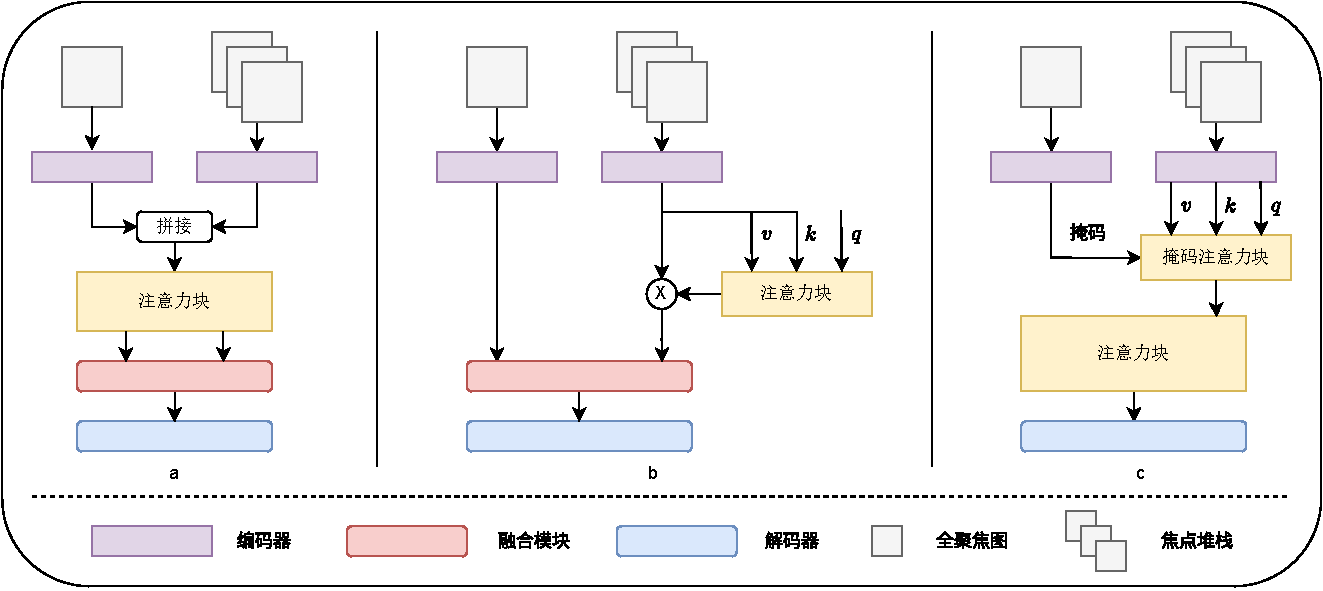
\includegraphics[width=0.95\linewidth]{figures/chapter4/task2_ins.drawio}
	\bicaption{光场显著性检测网络中不同的Transformer注意力机制}
	{Different Transformer attention mechanisms in light field saliency detection network}  
	\label{cpt4_fig1:task2_ins}
\end{figure}
%
%
%
%
王等人\upcite{wang2023tenet}通过拼接焦点堆栈和全聚焦图特征,
一并送入Transformer编码器来建立光场整体结构的感知模型。
如图~\ref{cpt4_fig1:task2_ins}~(a)~所示,
但是,这种方式弱化了全聚焦图片特征和散焦图片特征之间的模态差异,两个模态之间的融合依然依赖后续的融合模块。
刘等人\upcite{liu2023lftransnet}只在焦点堆栈支路使用了Transformer结构。该方法聚合多尺度的焦点堆栈特征构造注意力矩阵,用一个可学习的权重来作为查询矩阵。通过注意力运算来汇总不同切片对显著性检测的贡献。
网络结构如图~\ref{cpt4_fig1:task2_ins}~(b)~所示。
%
%
这种方法没有充分考虑两个模态之间的差异,仅在单焦点堆栈模态起到特征强化效果,只能考虑有限的特征表达。
% 
% 
% 
% 
\par
%
%
针对上述问题,本章提出一种基于视角增强的光场显著性目标检测方法。
此方法致力于从焦点堆栈和全聚焦图的协同感知入手,结合Transformer强大的注意力机制,提出了视角增强的注意力方法,网络结构如图~\ref{cpt4_fig1:task2_ins}~(c)~所示。
本章方法构建在一个简单的骨干网络之上,添加了视角增强编码器,
首先两个支路先进行交叉注意力计算,进行一个初步的互感知;
再用从焦点堆栈特征提取共有的显著性视角表达,注入到以全聚焦图为主的交叉注意力模块内,促进对全聚焦图的注意力权重向共有显著性表达迁移。
之后将全聚焦图的特征注入到焦点堆栈特征来增强每一张焦点堆栈图像的视角表达。
通过使用掩码注意力,注意力被限制在以全聚焦预测片段为中心的显著性特征上。
与标准的Transformer解码器中使用的交叉注意力(关注图像中的所有位置)相比,
被屏蔽的注意力能够达到更快的收敛效果和性能提高。
其次,为了进一并提高网络的表达能力,探索了使用基于图片像素的对比学习策略,
来引导网络学习差异化的显著性语义和背景语义信息。
%
%
\par
% 
% 
% 
% 
为验证本方法的有效性,本章在 DUTLF, LFSD 以及 HFUT-LFSD 数据集上进行了实验,
同样获得了超越其他光场显著性分割网络的性能,为光场数据的应用奠定了基础。
% 
% 
% 为了进一步验证本方法的有效性,本章将提出的数据增强方法应用在当前最
% 好的光场显著性检测方法上,实验结果表明,本章的数据增强方法能够提升其它方法的
% 检测性能。
% 
% 
% 在视角增强编码器中,使用了掩码注意力,将
% ~
% 随着
% 然而,采集光场数据需要多组摄像头或相机矩阵,造成了高昂的成本。为了实现理想的光场显著性目标检测能力,除了设计合适的网络模型外,还需要大量高质量的光场数据。由于光场数据获取成本高,目前的方法通常采用数据增强手段来增加训练数据。传统的数据增强方法包括旋转、平移、裁剪和缩放等操作,但这些方式的变化有限,效果也不够显著。对于不同类型的光场数据,需要不同的增强方法,选择不当的方法可能会引入噪声,导致训练不稳定,降低模型性能。因此,如何稳定生成高质量的光场数据以实现数据增强的目标是当前需要解决的问题。
% 针对上述问题。  
% % task2_ins.drawio







%%%%%%%%%%%%%%%%%%%%%%%%%%%%%%%%%%%%%%%%%%%%%%%%%%%%%%%%%%%%%%%%%%%%%%%%%%%%%%%%%%%%
\BiSection{方法介绍}{Method Introduction}
% 
% 
%
%
%
%
%
\begin{figure}[!ht]
	\centering
	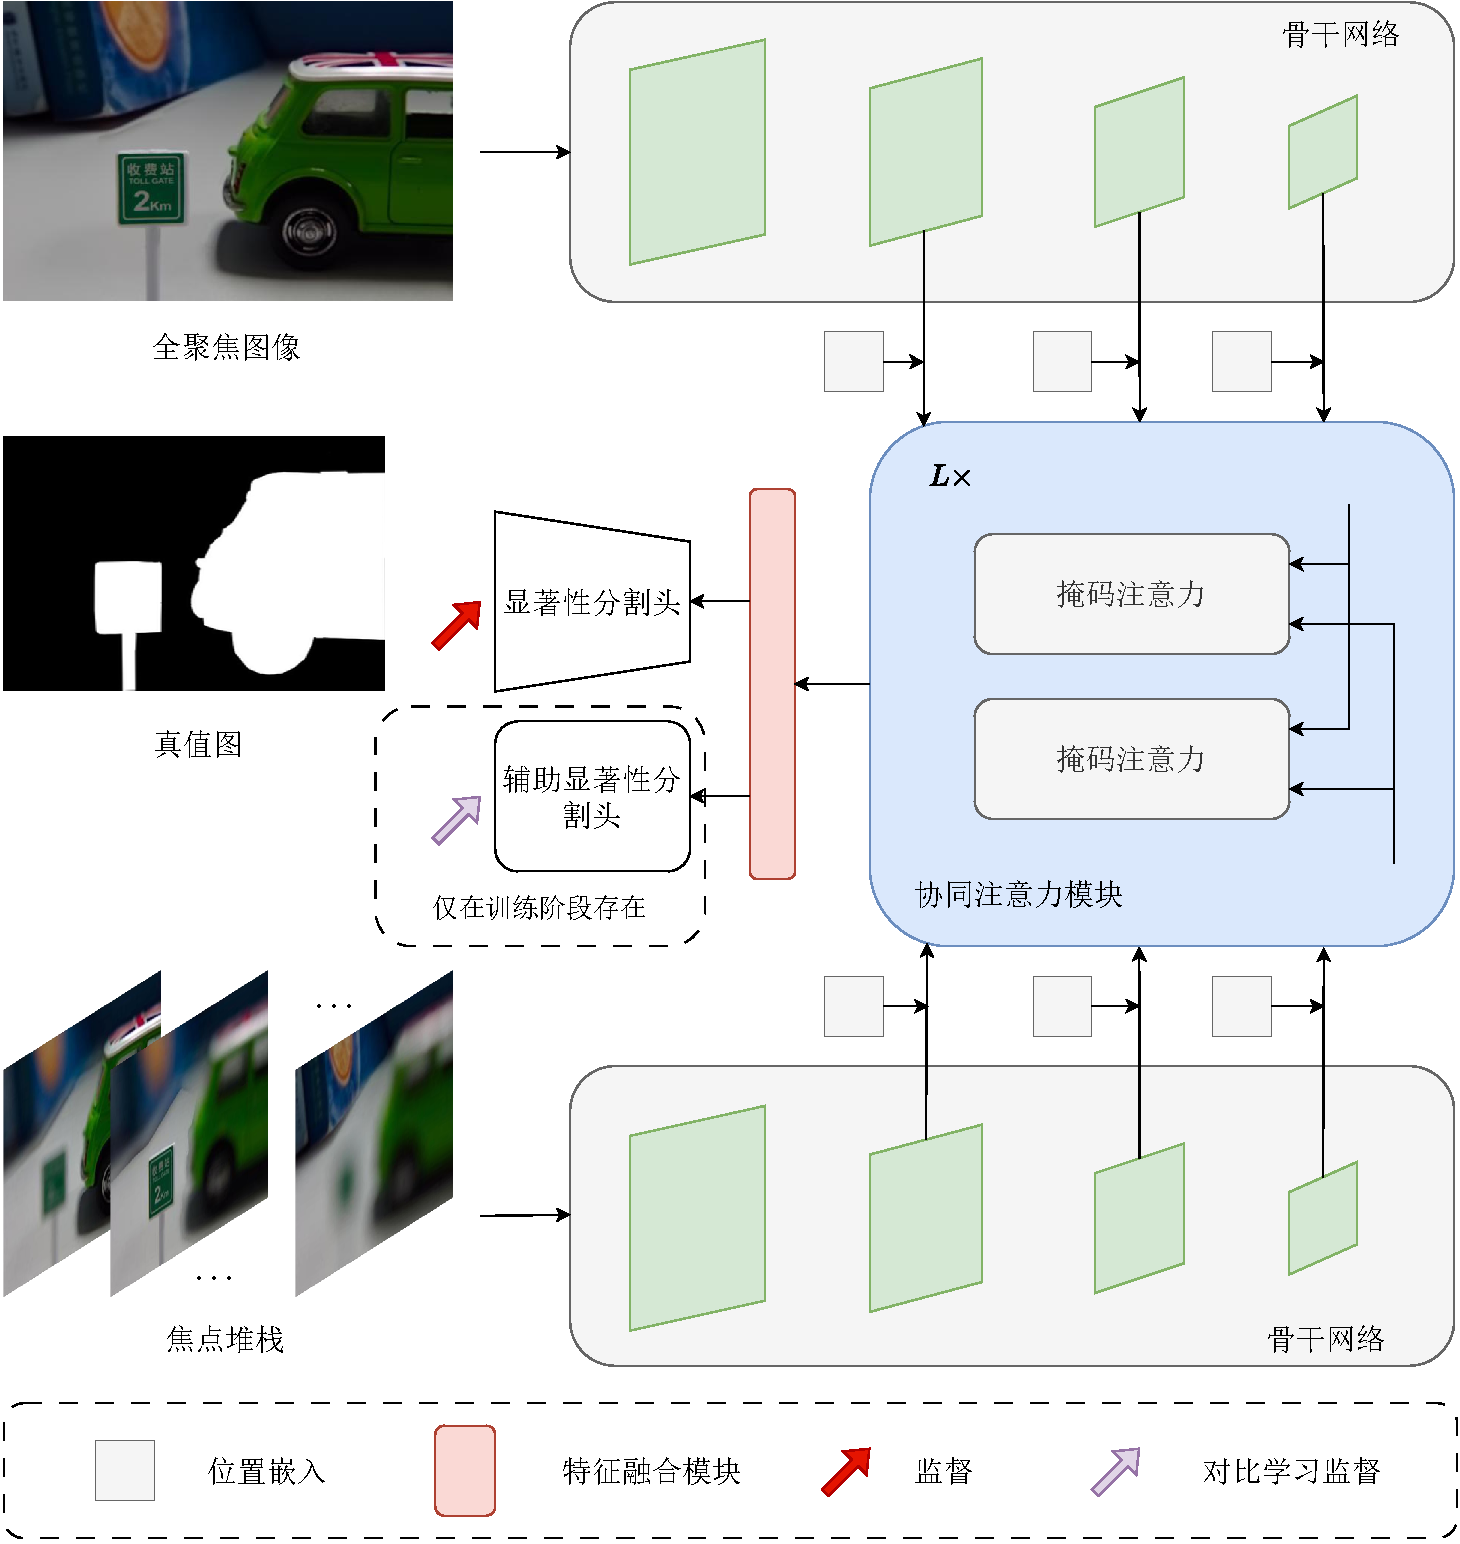
\includegraphics[width=0.95\linewidth]{figures/chapter4/chpt4_overview}
	\bicaption{基于视角增强的光场显著性目标检测网络}
	{Light field salient object detection network based on perspective enhancement}  
	\label{cpt4_fig1:chpt4_overview}
\end{figure}
%
%
%
%
%
本节将对本章提出的光场显著性目标检测网络模型进行详细介绍。
整体网络架构如图~\ref{cpt4_fig1:chpt4_overview}
~所示。
本章采用了在显著性目标检测任务中经常被使用的PVT-v2作为骨干网络。
具体来说,给定一个尺寸为$W \times H$的RGB图像$I_{0}$和
焦点堆栈$\left \{  I_{1},I_{2},I_{3},\cdots,I_{12} \right \} $,
分别输入编码器中以提取分辨率为$\frac{W}{2 \times 2^{l}} \times \frac{H}{2  \times 2^{l}} $ 
的特征$\left \{ F_{i}^{l},~l=1,2,3,4 \right \}$,
其中,$F_{i}^{l}$表示图像$I_{i}$在编码器第$l$层的特征,当$i=0$时,
$F_{i}^{l}$表示全聚焦图的特征,当$i=1,2,\cdots,12$时,$F_{i}^{l}$表示焦点堆栈图像的特征。
两个支路的编码器共享权重。由于使用注意力计算是图像尺寸的平方级复杂度,
本章方法只在特征尺度$\left \{ F_{i}^{l},~ l = 2, 3, 4\right \}$进行视角增强注意力计算。
增强后的全聚焦特征$ E_{0}^{l} $ 和焦点堆栈特征 $\left \{ E_{i}^{l},~i=1,~2,~ \cdots,~12 \right \}$
被送入特征融合模块,进行特征整合。
为了增强模型对显著性物体的辨识能力,本章方法采用了一个辅助显著性目标检测头,
用来生成对输入图片中不同像素位置的特征表示。并通过放大显著性前景区域与背景区域的差异,来辅助训练。
之后显著性分割头利用整合后的特征和骨干网络输出的第一层多尺度
特征$\left \{ F_{i}^{1},~i=0,~1,~ \cdots, ~12 \right \}$进行融合,并生成最终的显著性预测。
%
%
%
%
%参考CPD的建议,低阶特征由于太简单而无法做出有效且可靠的预测,
%本章只在高阶特征(即$F_{i}^{l},~j=2,3,4,5$)上执行解码操作。
%
%\textcolor{red}{TODO}
%
本章工作提出的视角增强模块和跨图的像素对比学习策略将
分别在~\ref{chap:part4_view_enh}~以及~\ref{chap:part4_cons}~节进行详细介绍。









%%%%%%%%%%%%%%%%%%%%%%%%%%%%%%%%%%%%%%%%%%%%%%%%%%%%%%%%%%%%%%%%%%%%%%%%%%%%%%%%%%%%
\BiSubsection{视角增强模块}{Viewpoint Enhancement Module}
\label{chap:part4_view_enh}


\begin{figure}[!ht]
	\centering
	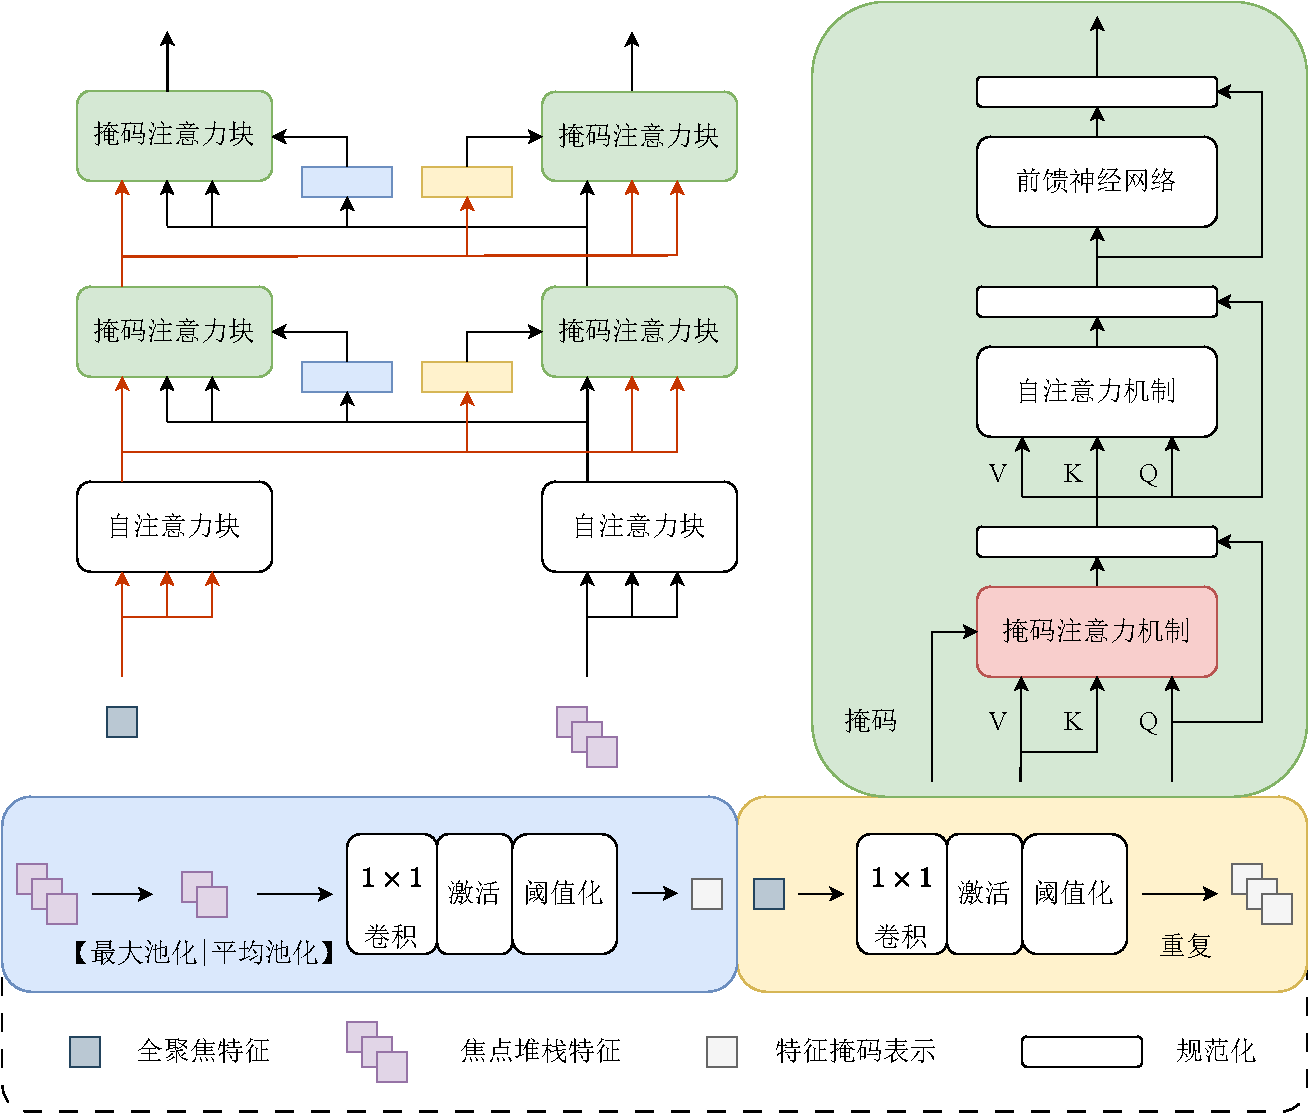
\includegraphics[width=0.95\linewidth]{figures/chapter4/view_enhance}
	\bicaption{视角增强注意力模块的框架流程图}
	{Framework diagram of the perspective-enhanced attention module}
%	{Perspective enhanced attention module}  
	\label{cpt4_fig1:view_enhance}
\end{figure}



视角增强模块综合考虑全聚焦图片的整体清晰视角和每一张焦点堆栈图片的局部清晰视角,
利用协同注意力的方式寻找全聚焦特征和焦点堆栈特征中对显著性目标检测最有效的语义信息。
视角增强注意最理想的情况是协同注意力权重往有效区域分布。
本节工作的目的是生成显著性视角表示,并对两个模态的互注意力权重进行加权以突出
显著性区域表示。


增强两个模态的特征表示,
一个直接的方式是使用全聚焦图和焦点堆栈的特征输入交叉注意力模块来强化特征,
但是,光场数据有限,模型容易陷入局部优化区。
并且,散焦区域特征和聚焦区域特征都是拍摄的同一场景,在特征层面相差不大,
互注意力模型在训练过程中往往迭代缓慢,且易生成较差的权重矩阵\upcite{piao2021panet}。
本章提出视角增强模块,通过在进行全聚焦特征和焦点堆栈特征
的交叉注意力权重时,使注意力限制在共有显著区域内部,
从而在特征整合中突出有效的聚焦显著性区域。


具体来说,
从共享权重的骨干网络中获取到四层特征$\left \{ F_{i}^{l},~l=1,2,3,4 \right \}$后,
考虑到Transformer块对于图像尺寸是一个平方级的计算复杂度,
使用越低级的语义信息,会带来更高的计算复杂度。
本章方法采取一种折中的办法,
只使用原始图像分辨率为$1/32,~1/16$和$1/8$的像素编码器产生的特征金字塔。
对于每一个分辨率,在输入到Transformer解码器之前加入正弦位置嵌入
$ e_{pos}\in \mathbb{R}^{H_{l}W_{l}\times C} $。
使用的Transformer解码器层,使用从次低分辨率到最高分辨率的三层特征,
如图~\ref{cpt4_fig1:chpt4_overview}~所示。
网络总共重复这个3层的Transformer解码器$L$次。因此,网络最终的Transformer解码器层有$3L$层。
更具体的说,前三层介绍分辨率$H_{1}=H/32,H_{2}=H/16,H_{3}=H/8$
和$W_{1}=W/32,W_{2}=W/16,W_{3}=W/8$的特征图,其中$H$和$W$是原始图像分辨率。
之后的所有层都以循环的方式重复此模式。



对全聚焦特征$ F_{0}^{4} $和
焦点堆栈特征$ \left \{ F_{i}^{4}, i=1,2, \cdots, 12 \right \}$
进行自注意力计算以增强其模态内的特征表示。
自注意力最早来源于Transformer架构\upcite{vaswani2017attention},
给定一个查询元素(例如,输出句子中的目标单词)和一组关
键元素(例如,输入句子中的源单词),多头注意力模块根据衡量查询密钥对兼容性
的注意力自适应地聚合关键内容。
为了使模型能够关注来自不同表示子空间和不同位置的内容,不同注意力头的输出与可学习的权重进行线性聚合。
%
%
%
%为了让模型关注来自不同子空间和不同位置的内
%容,不同注意力头的输出与科学系的权重进行线性聚合。
%
%
%
%Transformer 中的多头注意力。
%Transformer最早用于机器翻译的,是一种基于注意力机制的网络架构。
%给定一个查询元素(例如,输出句子中的目标单词)和
%一组关键元素(例如,输入句子中的源单词),
%多头注意力模块根据衡量查询密钥对兼容性的注意力自适应地聚合关键内容。
%为了让模型关注来自不同子空间和不同位置的内容,不同注意力头的输出与科学系的权重进行线性聚合。
%
%
%
令$q\in \Omega_{q}$索引具有表示特征$z_{q} \in \mathbb{R}^{C}$的查询元素,
$k\in \Omega_{k}$索引具有表示特征$x_{k} \in \mathbb{R}^{C}$的关键元素,
其中$C$是特征维度,$\Omega_{q}$和$\Omega_{k}$分别指定查询元素和关键元素的集合。
然后计算多头注意力特征的公式如下:
% 
% 
% 
% 
\begin{equation}
	MultiHeadAttn(z_{q},~x)=\sum_{m=1}^{M}
	W_{m}\left [ ~~\sum_{k\in \Omega_{k}}^{}A_{mqk} ~\cdot~ W_{m}^{'} x_{k}  ~~\right ]  
\end{equation}
% 
% 
% 
% 
其中$m$是注意力头的索引,
$ W_{k}^{{}' } \in \mathbb{R}^{C_{v} \times C} $
和$W_{m} \in \mathbb{R}^{C\times C_{v} }$
是可学习的权重(默认情况下$C_{v}=C/M$)。
注意力权重 
$A_{mqk} \propto exp \left \{ 
\frac{
	z_{q}^{T} U_{m}^{T} V_{m} x_{k}
}{ \sqrt{C_{v}}
}  \right \} $
% 
% 
% 
归一化为$ {\textstyle \sum_{k\in\Omega_{k}}^{}} A_{mqk} = 1$,
其中$U_{m},~V_{m} \in \mathbb{R}^{C_{v}\times C}$也是可学习权重。
为了消除不同空间位置的歧义,表示特征$z_{q}$和$x_{k}$通常是元素内容和位置嵌入的串联求和。





但是,只进行模态内部的自注意计算,无法感知到隐含在焦点堆栈内部的三维场景信息。
还需要焦点堆栈和全聚焦图像进行互相的特征增强,其他的特征融合增强的范式可以见图~\ref{cpt4_fig1:task2_ins}。
最近的研究\upcite{gao2021fast,sun2021rethinking}表明,
基于Transformer的模型收敛缓慢是由于交叉注意力层中的全局上下文,
因为交叉注意力需要许多训练周期才能学会关注局部对象区域\upcite{sun2021rethinking}。
局部特征足以更新查询特征,并且可以通过自注意力收集上下文信息\upcite{cheng2022masked}。
标准的交叉注意力(带残差路径)计算公式如下:
\begin{equation}
	X_{l}=Softmax(Q_{l}K_{l}^{T})V_{l} + X_{l-1}
\end{equation}
其中,$l$是层索引,$X_{l} \in \mathbb{R}^{N\times C}$
是指在$l^{th}$层和
$ Q_{l} = f_{Q} \left ( X_{l-1} \right ) \in \mathbb{R}^{N \times C} $
的维度查询特征。$X_{0}$表示Transformer解码器的输入查询特征。
$K_{l},V_{l} \in \mathbb{R}^{H_{l}W_{l} \times C}$
分别表示经过$f_{K}(\cdot) $和$ f_{V}( \cdot )$变换后的
输入图像特征,
$H_{l}$和$W_{l}$是图像特征的空间分辨率。
$f_{Q} (\cdot),~f_{K}(\cdot) $和$ f_{V}(\cdot) $是线性变换。
$ Softmax(\cdot) $ 函数将输入的权重矩阵映射为 $(0,~1)$之间的分布,
并且使得输出值的累计和为1,从而满足概率性质,即对概率最大的元素加强注意。
%
%
%
%
%
\par
%
%
%
%
这些问题在光场中会更加严重。
在光场中应用交叉注意力机制,
会使得注意力权重往散焦图片中清晰的部分偏移,
因为散焦图片中既有前景清晰的部分,也有背景清晰的部分,
网络很容易被背景清晰的部分误导,从而产生错误的显著性预测结果。
且网络需要更多的迭代训练才能对是否是前景显著物体有一个很好的辨识度。
%
%
%
%
%
\par
%
%
%
%
针对上述注意力弥散的问题,
本节提出掩码交叉注意力,可以看做是交叉注意力机制的一种变体,
仅关注每个查询的预测掩码的前景区域内。
% 
% 
% 
% 
掩码注意力通过以下方式调节注意力矩阵:
\begin{equation}
	X_{l}=softmax(M_{l-1} ~+~Q_{l}K_{l}^{T})V_{l} + X_{l-1}
\end{equation}
% 
% 
此外,在特征位置$(x,~y)$的注意力掩码$M_{l-1}$是从另一个模态的特征提取的共有表示。
%
%
%
%
%
%
\par 
%
%
%
%
根据交叉注意力的方式不同,注意力掩码有两个生成方式,
对于全聚焦图特征$F_{0}^{l}$与焦点堆栈特征的交叉注意力,
使用来自焦点堆栈的共有表示来强化注意力权重。
对于给定焦点堆栈特征$\left \{ F_{i}^{l}, i=1,2,\cdots, 12 \right \}$,
进行如下变换:
%
%
%
%
\begin{equation}
\begin{aligned}
	\hat{F} &= Concat(\left [  F_{1}^{l}, F_{2}^{l}, \cdots, F_{12}^{l} \right ] ) \\
	M_{a}^{l} &= \bar{f}
	\left (  \sigma \left ( f^{1 \times 1}\left [  
	AvgPool\left ( \hat{F} \right ) ,~ MaxPool\left ( \hat{F} \right ) 
	\right ]  \right )  \right )
\end{aligned}
\end{equation}
%
%
%
其中$Concat(\cdot)$表示在通道维度进行拼接操作,
$\sigma(\cdot)$表示RELU激活函数,
$f^{1\times 1}$表示$1\times 1$通道卷积操作,
$AvgPool(\cdot)$
和$MaxPool(\cdot)$
分别表示通道维度上的平均池化和最大池化操作。
$\bar{f}$表示将得到的掩码进行阈值化处理,公式如下:
%
%
%
%
%
%
%
\begin{equation}
M^{l}\left ( F\left ( x, ~y \right )  \right ) =
\begin{cases}
	0  & \text{ if } ~~ F(x,~y)>  \alpha \\
	-\infty & \text{ otherwise } 
\end{cases}
\end{equation}
%%
%
%
%
其中$\alpha$是超参数,是对特征进行二值化的阈值,一般设为0.5。
%
%
%
%
%
%
\par
%
%
%
%
%
而对于焦点堆栈支路的掩码交叉注意力计算,
掩码使用来自全聚焦特征支路的特征表示来生成共有表示,其公式如下:
%
%
%
%
\begin{equation}
	M_{fs}^{l} = \bar{f}   \left ( \sigma \left ( 
	f^{1\times 1}
	\left ( 
%	\hat{F}
	F_{0}^{l}
	\right ) 
	\right )   \right ) 
\end{equation}
%
%
%
%
其注意力计算的的 $Q_{l}$ 是  $ \hat{F}$,
$K_{l}$ 
和
$V_{l}$是来自全聚焦支路的特征 $F_{0}^{l}$。
%
%
%
%
%
\par
%
%
%
%
语义分割任务中,上下文特征已经被证明对图像分割很重要
\upcite{chen2017deeplab,chen2017rethinking,zhao2017pyramid},
高分辨率的语义特征对提高模型性能具有显著帮助,特别是小物体的分割。
本章方法在特征融合阶段对于骨干网络中获取的最低尺度特征$\left \{ F_{i}^{0}, i = 0, 1, \cdots, 12 \right \}$加以考虑。
特征融合模块获取
视角增强模块的输出$\left \{ E_{i}^{l}, i = 0, 1, \cdots, 12 \right \}$
和最高分辨率的语义特征。具体的融合过程如下:
%
%
%
%
\begin{equation}
	\begin{aligned}
		E^{l+1} &= 
		Concat\left ( \left [ E_{0}^{l+1},E_{1}^{l+1},\cdots, E_{12}^{l+1} \right ]  \right )  
		\\  
		F^{l} &= 
		Concat\left ( \left [ F_{0}^{l},F_{1}^{l},\cdots, F_{12}^{l} \right ]  \right )  
		\\  
		{O^{l}}  &= Conv\left (  Upsample\left ( f^{3 \times 3} \left ( E^{l+1} \right )  \right ) + F_{0}^{l} \right )  \\
	\end{aligned}
\end{equation}
%
%
%
%
其中,$Concat(\cdot)$是通道拼接操作,
$f^{3 \times 3}$ 是 $3 \times 3 $ 卷积操作,
$ Upsample(\cdot) $ 是2倍上采样过程,
$ Conv $ 是一个组合操作,包含 $3\times 3$卷积、批归一化和RELU激活函数。
特征融合模块从高层语义特征汇总到低层语义信息,
层级表示$i$的取值依次为$\left \{ 3,2,1 \right \}$。
%
%
%
%
%
\par 
%
%
最后将获取到的融合模块的输出特征$\left \{ O^{l}, l = 1,2,3 \right \}$
送到显著性分割头进行最终的分割预测 $P$,
同时,为了增强网络的表示,本章方法采用多尺度监督,
分别在图像尺寸为1/16、1/8和1/4的原图像尺寸上预测显著性图
$\left \{ P^{l}, l = 1,2,3 \right \}$。
具体来说,采用如下公式:
%
%
%
%
\begin{equation}
	P^{l} = \sigma \left ( Conv\left ( MaxPool \left (  
	O^{l} \right )  \right )  \right ) 
	\times 
	O^{l} + O^{l},~ l = 1,2,3
\end{equation}
%
%
%
%
其中,$MaxPool(\cdot)$是通道维度的最大池化操作,
$ Conv $ 表示 $ 3\times 3 $卷积操作,
$ \sigma $ 代表的是 RELU 激活函数。
获取到的三个显著性预测图分别以真值图进行监督训练,
显著性分割损失
$ \mathcal{L}_{sal} $
定义为:
%
%
%
%
\begin{equation}
	\mathcal{L}_{sal} = \sum_{l = 1}^{3}  
	\mathcal{L}_{bce} \left ( P^{l}, DownSample_{j}\left (  GT \right ) 
	\right ), ~ j = 2\times 2^l
	\label{chpt4:eq:loss_sal}
\end{equation}
%
%
%
%
其中$\mathcal{L}_{bce}$ 表示二值交叉熵损失函数,
$DownSample_{j}(\cdot)$ 表示将输入下采样$j$ 倍。
%
%
%
%
%
\BiSubsection{感知对比学习策略}{Contrastive Perception Learning Strategy}
\label{chap:part4_cons}
% 
% 
% 
% 
显著性目标检测网络一般使用$sigmoid$ 作为输出结果的映射头,
这种通过阈值化分割前景和背景的方式,
虽然能够通过交叉熵损失优化前景和背景中每个像素点与真值预测图之间的距离,
但忽略了像素之间的关系\upcite{zhao2019region},
在一些置信度低的区域,比如前背景相似的像素区域,
网络容易产生错误的预测,或者在学习不到位时,会预测出虚影。
%
%
%
%
虽然显著性分割是一个像素级的分类任务,但是每张图像的前景区域内部和背景区域内部也是有差异所在。

在本章工作中,构造了一种逐像素对比学习的方法,
通过规范嵌入空间并探索训练数据的全局结构来解决上述问题。
使得网络能够在做出像素级显著性分割预测时,也能够考虑同类像素之间的关系,
学习显著性区域内部的一致性表达,
和背景区域内部的一致性表达,在光场显著性目标检测领域引入了
感知对比学习。



对比学习常用于无监督中视觉表示学习。
无监督对比学习旨在学习CNN编码器$f_{CNN}$将每个训练图像转换为特征向量表示$v=f_{CNN}(I) \in \mathbb{R}^{D}$,
使得$v$能够描述图片$I$。
为了实现这一目标,
对比学习通过区分正样本(一个增强版本的图像$I$)
和多个负样本(从训练集中随机挑选的图像,但是不包括$I$)来进行训练。
在对比学习中,会集成使用InfoNCE损失函数,其公式如下:
\begin{equation}
	\mathcal{L} _{NCE}^{I}=-log \frac{exp(v \cdot v^{+ }/\tau )}
{exp(v \cdot v^{+}/\tau )+ \sum_{v^{-}\in N_{I}} exp(v \cdot v^{-}/\tau )} 
\label{chpt4_equ_nce}
\end{equation}
其中$v^{+}$是正样本图像$I$的嵌入,$N_{I}$是包含负样本的嵌入,$\cdot$表示内(点)积,
$\tau >0$是温度超参数。损失函数在计算前,还需要对所有嵌入进行$\ell_{2}$归一化。
\par
% 
% 
% 

% 

在显著性分割的背景下,图像$I$的每个像素$i$需要被分类为显著性的前景类或者背景类。
当前的方法通常将此任务视为逐像素分类问题。具体来说,
令$f_{FCN}$作为图像特征编码器(例如ResNet\upcite{he2016deep}),它为图像$I$生成密集特征预测
$I\in \mathbb{R}^{ H \times W \times D}$,
从中可以导出每个像素的嵌入$i \in  \mathbb{R}^{D}$。



本章方法首先扩展了公式~\ref{chpt4_equ_nce},
去适配网络模型有监督的密集图像预测任务。
总的来说,本章方法的对比损失函数计算的是数据样本中每张图像的像素。
对于具有真实语义标签的像素$i$,正样本是也属于该类的其他像素,
而负样本是属于其他类的像素。
本章的有监督形式的逐像素对比损失定义为:


\begin{equation}
	\mathcal{L} _{NCE}^{I}= 
	\frac{1}{|P_{i}|}
	\sum_{i^{+}\in P_{i}}^{}  
	-log \frac
	{exp(i \cdot i^{+ }/\tau )}
	{exp(i \cdot i^{+}/\tau )+ \sum_{i^{-}\in N_{I}} exp(i \cdot i^{-}/\tau )} 
	\label{chpt4:eq:con_loss}
\end{equation}



% =======
其中$P_{i}$和$N_{i}$分别表示像素$i$的正样本和负样本的像素嵌入集合。
并且,正负样本和锚点$i$不局限于统一图像。如公式~\ref{chpt4:eq:con_loss}~所示,
这种基于像素到像素对比度的损失设计的目的是通过
将同一类像素样本拉进
并
将不同类像素样本推开来学习其隐含的嵌入表示。





% 
% 
公式~\ref{chpt4:eq:loss_sal}~中的像素二元交叉熵损失
$\mathcal{L}_{sal} $
以及
在公式~\ref{chpt4:eq:con_loss}~中的对比损失
$\mathcal{L}_{NCE} $
是互补的。
前者能让显著性分割网络学习对前背景分类有意义的判别性像素特征,
而后者通过显示探索像素样本之间的全局语义关系,
有助于规范嵌入空间,
提高类内紧凑性和类间可分离性。
因此总体训练目标是:
\begin{equation}
	\mathcal{L}_{total} = \sum_{i}^{} \mathcal{L}_{sal}^{i} + \mathcal{L}_{NCE}^{i}
%	\mathcal{L}^{SEG}=\sum_{i}\left ( 
%	\mathcal{L}_{i}^{CE} + 
%	\lambda \mathcal{L}_{i}^{NCE}  
%	\right ) 
\end{equation}
% 
% 
% 
% 
其中$\lambda > 0 $是系数,$\mathcal{L}^{total}$
学习到的像素嵌入变得更加紧凑且分离良好。
这表明,通过利用二元交叉熵损失和成对比度量损失的优势,
显著性分割网络可以生成更具辨别力的特征,
从而产生更有希望的结果。









%%%%%%%%%%%%%%%%%%%%%%%%%%%%%%%%%%%%%%%%%%%%%%%%%%%%%%%%%%%%%%%%%%%%%%%%%%%%%%%%%%%%%%%%%%
\BiSubsection{训练过程}{Training Process}



本文中提到的
感知对比表示头,如图~\ref{cpt4_fig1:chpt4_overview}~中所示,
和对比损失 $\mathcal{L}_{NCE}$
只在训练过程中存在。
在测试阶段,使用显著性分割头预测的最后一个预测 $P^{1}$, 再通过双线性插值到原图大小后,
经过$sigmoid(\cdot)$激活后作为最终的显著性分割预测。




%%%%%%%%%%%%%%%%%%%%%%%%%%%%%%%%%%%%%%%%%%%%%%%%%%%%%%%%%%%%%%%%%%%%%%%%%%%%%%%%%%%%%%%%%%%%
\BiSection{实验结果与分析}{Experimental Results and Analysis}

\BiSubsection{实验设置}{Experimental Setup}
(1)数据集

本章在 3 个公开的光场数据集:
DUT-LFSD\upcite{zhang2019memory}、
HFUT-LFSD\upcite{zhang2017saliency}以及 
LFSD\upcite{li2014saliency}上
进行了大量的实验。DUT-LFSD 包含 1462 张光场样本,HFUT-LFSD 包含 255 个样本,
LFSD 包含 100 个光场样本。每个样本包含一个 RGB(全聚焦)图像,焦点堆栈以及一
个像素级的显著性真值。本章采用了与 ERNet\upcite{piao2020exploit}相同的训练集。具体来说,本章从
DUT-LFSD 中选择了 1000 个样本,并从 HFUT-LFSD 中选择了 100 个样本作为训练集。

(2)实现细节

本章的方法是在 Pytorch 框架上实现的,并使用单个 GTX2080Ti 的显卡进行训练。在训
练过程中,本章使用 AdamW 优化器,并将优化器中的动量以及权重衰减参数设置为 0.9
以及 0.00005。
优化器的学习率设置为 3e-5,并在前 5 万次迭代过程中逐渐衰减并最终
衰减为原学习率的 1/10。
小批量尺寸大小设定为 2,并将网络中批量归一化(BatchNorm, BN)修改为组
归一化 (GroupNorm,GN)。
最大迭代次数设置为 10 万次,所有光场数据大小均调整到 256×256后进行训练和测试。

(3)评价指标

为了公平的比较不同网络的性能,本章采用了 S-measure、E-measure、F-measure、绝对平均误差MAE作为评
估模型性能的指标。




%%%%%%%%%%%%%%%%%%%%%%%%%%%%%%%%%%%%%%%%%%%%%%%%%%%%%%%%%%%%%%%%%%%%%%%%%%%%%%%%%%%%%%
\BiSubsection{消融实验}{Ablation Experiment}


\begin{table}[!hb]
	\bicaption{在DUTLF-FS数据集上每个组件的消融实验分析}
	{Ablation experimental analysis of each component on the DUTLF-FS dataset}
	\centering
	\label{chpt4:tab:abl_tot}
	%	\resizebox{0.82\linewidth}{!}{
		\begin{tabular}{lcccccccc}
			\toprule[2pt]  %添加表格头部粗线
			%%  \multicolumn{1}{c}{ \multirow{2}*{Methods} }
			
			\multicolumn{1}{c}{ \multirow{2}*{模型设置}}	& \multicolumn{4}{c}{DUTLF-FS} & \multicolumn{4}{c}{HFUT} \\ 
			
			%			\cmidrule(r){2-9} 
			
			\cmidrule(r){2-5} \cmidrule(r){6-9} 
			
			& $E_{\phi}^{max}\uparrow$ & $S_{\alpha }\uparrow $ & $F_{\beta}^{max}\uparrow$ & MAE$\downarrow$ 
			& $E_{\phi}^{max}\uparrow$ & $S_{\alpha }\uparrow $ & $F_{\beta}^{max}\uparrow$ & MAE$\downarrow$
			\\
			
			\midrule
			
			%			% 开始填写数据
			%			\multicolumn{2}{l}{ Baseline }     & 0.947 & 0.894 & 0.901 & 0.048 \\ 
			%			
			%			\midrule
			
			基础网络     & 0.959 & 0.918 & 0.926 & 0.037 & 0.876 & 0.822 & 0.781 & 0.069   \\
			+视角增强模块 & 0.968 & 0.933 & 0.944 & 0.027 & 0.873 & 0.828 & 0.788 & 0.061   \\
			
			
%			+像素对比学习 & \textbf{0.969} & \textbf{0.938} & \textbf{0.948} & \textbf{0.024} & \textbf{0.898} & \textbf{0.848} & \textbf{0.827} & \textbf{0.055}   \\
			
			+像素对比学习
			& \textbf{0.971} & \textbf{0.940} & \textbf{0.949} & \textbf{0.022} 
			& \textbf{0.902} & \textbf{0.852} & \textbf{0.823} & \textbf{0.052}  
			\\
			
			
			\bottomrule[2pt]
		\end{tabular}
		% }
\end{table}




%------------------------------ figure: comparison
\begin{figure}[!ht]
	\centering
	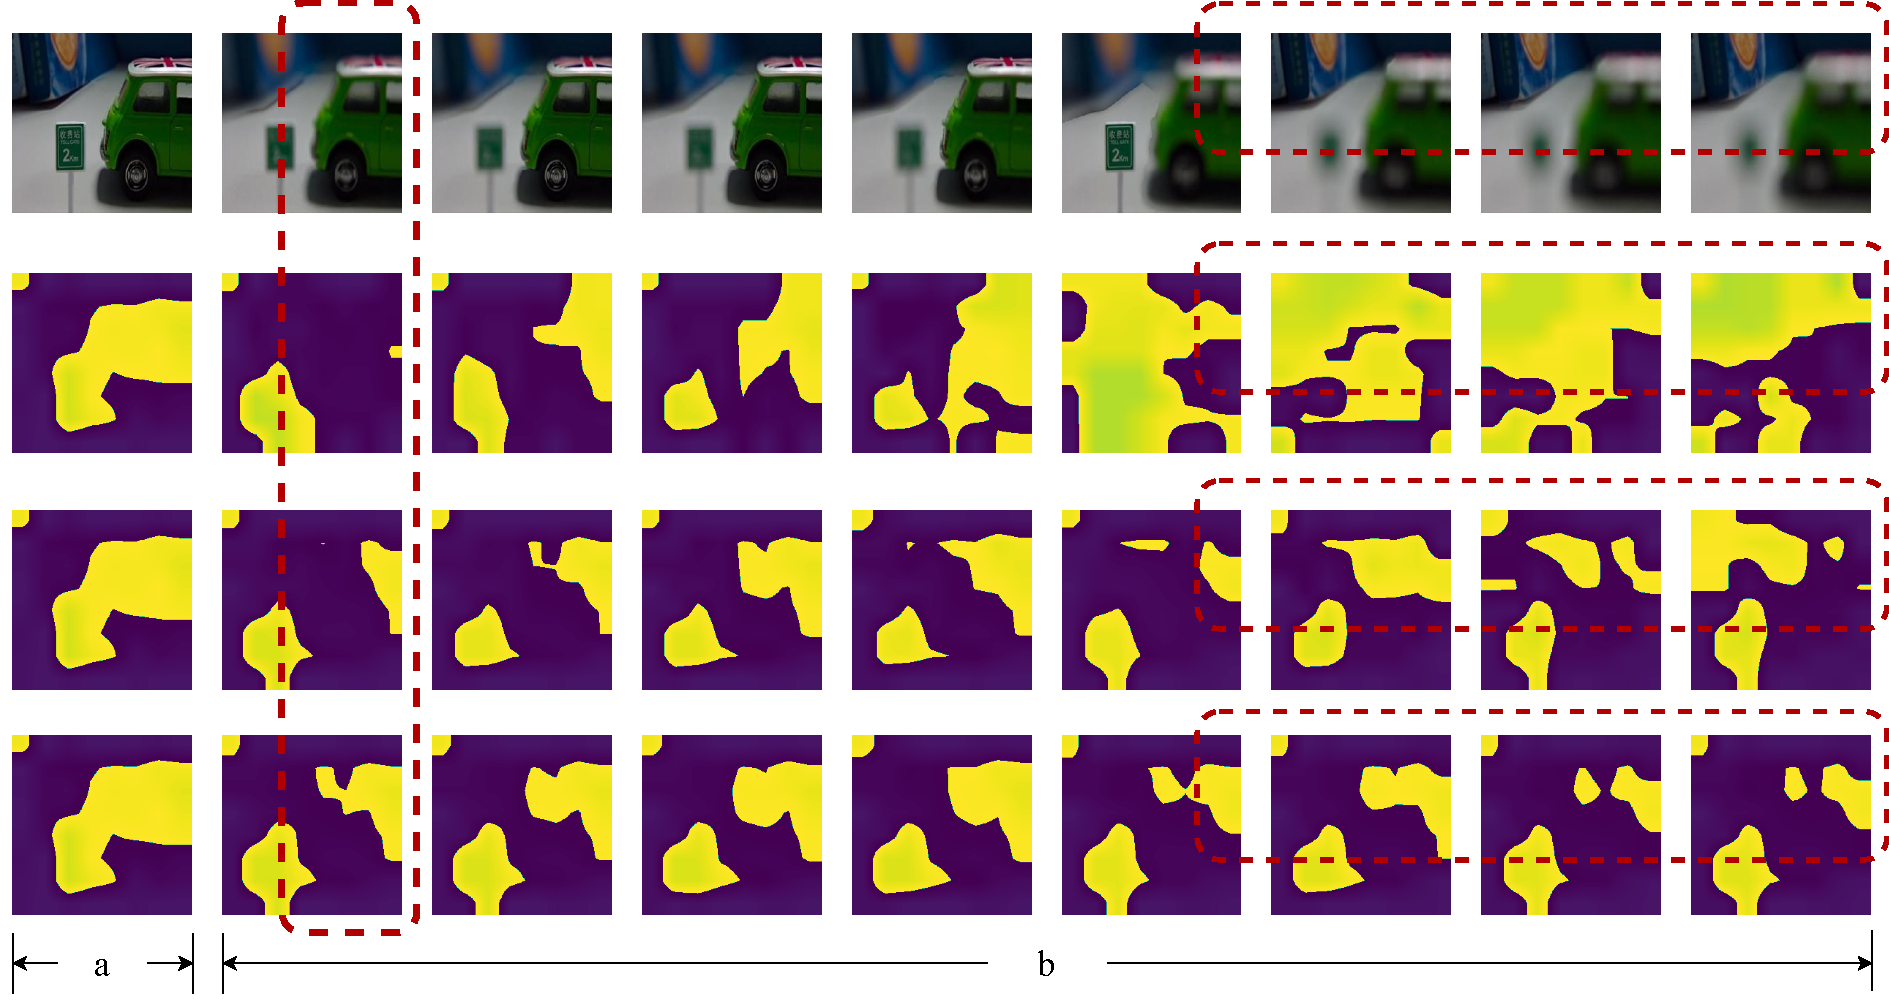
\includegraphics[width=\linewidth]{figures/chapter4/attn_show}
	\bicaption{视角增强注意力模块的可视化分析}
	{Visual analysis of perspective-enhanced attention module}
%	{不同交叉注意力机制的可视化分析}
%	{在一些具有挑战性的场景中与最先进的方法进行定性比较}
%	{Qualitative comparisons of state-of-the-art methods in some challenging scenes}
	\label{chpt4:figure:attn_show}
\end{figure}


\begin{table}[!ht]
	\bicaption{视角增强注意力模块的消融实验结果}
	{Ablation experimental results of perspective-enhanced attention module}
	\centering
	\label{chpt4:tab:abl_attn}
	%	\resizebox{0.82\linewidth}{!}{
		\begin{tabular}{lcccccccc}
			\toprule[2pt]  %添加表格头部粗线
			%%  \multicolumn{1}{c}{ \multirow{2}*{Methods} }
			
			\multicolumn{1}{c}{ \multirow{2}*{模型设置}}	& \multicolumn{4}{c}{DUTLF-FS} & \multicolumn{4}{c}{HFUT} \\ 
			
			%			\cmidrule(r){2-9} 
			
			\cmidrule(r){2-5} \cmidrule(r){6-9} 
			
			& $E_{\phi}^{max}\uparrow$ & $S_{\alpha }\uparrow $ & $F_{\beta}^{max}\uparrow$ & MAE$\downarrow$ 
			& $E_{\phi}^{max}\uparrow$ & $S_{\alpha }\uparrow $ & $F_{\beta}^{max}\uparrow$ & MAE$\downarrow$
			\\
			
			\midrule
			
			%			% 开始填写数据
			%			\multicolumn{2}{l}{ Baseline }     & 0.947 & 0.894 & 0.901 & 0.048 \\ 
			%			
			%			\midrule
			
			
			+自注意力 
			& 0.964 & 0.926 & 0.935 & 0.031 
			& 0.881 & 0.833 & 0.797 & 0.065   \\
			
			+交叉注意力
			& 0.965 & 0.931 & 0.943 & 0.027 
			& 0.881 & 0.833 & 0.795 & 0.060   \\
			
			+自掩码注意力  
			& 0.965 & 0.935 & 0.944 & 0.025 
			& 0.894 & 0.849 & 0.821 & 0.058   \\
			
			+掩码注意力   
			& \textbf{0.971} & \textbf{0.940} & \textbf{0.949} & \textbf{0.022} 
			& \textbf{0.902} & \textbf{0.852} & \textbf{0.823} & \textbf{0.052}  \\
			
			\bottomrule[2pt]
		\end{tabular}
		% }
\end{table}




在本小节,对提出的各个模块进行消融实验,
分析每个组件或者策略对于显著性分割性能的影响。
定量的消融实验结果展示在表~\ref{chpt4:tab:abl_tot}~中,
定性的消融实验结果展示在图~\ref{chpt4:figure:attn_show}~中。



(1)
验证视角增强模块的有效性


本章提出的视角增强模块是利用在进行交叉注意力计算时注入显著性表示,
使得交叉注意力权重能够合理分布。
为来证明视角增强注意力模块的有效性,本章设计了在只包含基线网络和融合模块的
基础上,逐渐添加视角增强注意力机制的组成部分,具体消融实验如
表~\ref{chpt4:tab:abl_attn}~
中所示。
首先在基线模型中,引入了自注意力机制来增强焦点堆栈和全聚焦两个模态的特征表示,
自注意力机制只在最高语义特征层添加,实验结果见表中第一行数据;
为了跨模态的信息传递,本章方法在第二和第三语义特征层添加了交叉注意力计算,
实验结果见表中第二行数据。
为了应对交叉注意权重根据散焦图片不同清晰部分而弥散的问题,
本章方法设计了使用显著性掩码表示来限制交叉注意力权重的视角增强方法,
表中第三行表示使用来自自身模态的显著性掩码表示来增强交叉注意力,
表中第四行表示使用来自跨模态的显著性掩码表示来增强交叉注意力权重。
本章方法在使用掩码交叉注意力机制时,取得了最好的性能,
这也说明来相较于只使用交叉注意力机制进行跨模态融合,
本章提出的基于显著性掩码表示的交叉注意力更能有效的从光场数据中探索显著性语义,
本章所提出的掩码注意力更加合理。



为了定性展示本章所使用的视角增强模块的有效性,
可视化了使用全聚焦图特征和焦点堆栈特征进行交叉注意力计算的权重图,
如图~\ref{chpt4:figure:attn_show}~所示,
其中(a)表示全聚焦支路,(b)表示焦点堆栈支路。
图中第一行是原始RGB图片,第二行是只使用交叉注意力机制生成的权重图,
特征使用的是骨干网络输出的最高层语义特征,经过注意力机制计算后,
使用双线性插值方法到原图大小后进行可视化。
第三行代表的是添加视角增强的掩码交叉注意力机制后的特征图;
第四行代表的是在进行掩码注意力时,使用交叉支路的掩码表示来互相增强权重后的可视化效果。
在图中,使用了红色的虚线框对差异部分进行着重表示。
左侧第二列的虚线框表示,只使用交叉注意力时,
只能注意到当前焦点切片图片中与全聚焦图共清晰的部分。
更多样例如第二行所示,在后几张焦点切片图片中,
交叉注意权重矩阵偏向场景中背景清晰的部分,给网络带来了误导的注意权重,
不利于网络学习显著性语义信息。
而通过添加掩码交叉注意力机制,如图中第二列所示,本来只注意到标志牌的权重特征,
开始逐渐注意场景中绿色的汽车,并注意向两个共有的显著性语义靠拢。
图中倒数三列,原始交叉注意力的权重更多的分布在共清晰的背景语义上,
通过掩码交叉注意力机制,
非显著的背景语义信息被逐渐抑制,并使得权重矩阵向着共显著性语义信息累计。
通过比较可视化特征图,展示了本章所提出的基于视角增强的掩码交叉注意力机制的有效性。






(2)
验证像素对比监督的有效性

为了验证像素对比监督策略的有效性,
本章在基线网络的基础上,去掉像素对比学习头,并且只使用二元交叉熵损失进行监督,
实验数据如表~\ref{chpt4:tab:abl_loss}~中第一行所示。
之后添加对比学习头,并使用像素对比学习损失加以监督,
实验结果见表中第二行,可以看到在DUTLF数据集上
S-measure和F-measure分别提升了0.6\%和0.9\%。
证明了本章像素对比监督方法对提升显著性网络预测精度的有效性。



\begin{table}[!hb]
	\bicaption{感知对比学习策略的消融实验}
	{Ablation experiments on perceptual contrast learning strategies}
	\centering
	\label{chpt4:tab:abl_loss}
	\resizebox{\linewidth}{!}{
		\begin{tabular}{lcccccccc}
			\toprule[2pt]  %添加表格头部粗线
			%%  \multicolumn{1}{c}{ \multirow{2}*{Methods} }
			
			\multicolumn{1}{c}{ \multirow{2}*{模型设置}}	& \multicolumn{4}{c}{DUTLF-FS} & \multicolumn{4}{c}{HFUT} \\ 
			
			%			\cmidrule(r){2-9} 
			
			\cmidrule(r){2-5} \cmidrule(r){6-9} 
			
			& $E_{\phi}^{max}\uparrow$ & $S_{\alpha }\uparrow $ & $F_{\beta}^{max}\uparrow$ & MAE$\downarrow$ 
			& $E_{\phi}^{max}\uparrow$ & $S_{\alpha }\uparrow $ & $F_{\beta}^{max}\uparrow$ & MAE$\downarrow$
			\\
			
			\midrule
			
			
			
			二元交叉熵损失   & 0.965 & 0.931 & 0.943 & 0.027 & 0.885 & 0.840 & 0.810 & 0.056  \\
			像素对比学习损失 			
			& \textbf{0.971} & \textbf{0.940} & \textbf{0.949} & \textbf{0.022} 
			& \textbf{0.902} & \textbf{0.852} & \textbf{0.823} & \textbf{0.052}  \\
			
			\bottomrule[2pt]
		\end{tabular}
	}
\end{table}



%
%
\begin{table}[!ht]
	\centering
	\label{chpt4:table:comp_with_sota_3_1}
	\bicaption{在3个光场公开数据集上与现有方法的定量比较}
	{Quantitative comparison with existing methods on 3 light field public datasets}
%	{在3个光场数据集上与现有方法的定量比较}
%	{Quantitative comparison with existing methods on 3 light field datasets}
%	{在 3 个公开数据集上的定量比较}
%	{Quantitative comparisons on three light field datasets}
	\resizebox{\textwidth}{!}{
		\begin{tabular}{rcccccccccccc}
			\toprule[2pt]  %添加表格头部粗线
			
			% title
			%			\multirow{2}*{Type} & 
			\multicolumn{1}{c}{ \multirow{2}*{方法} } & 
			\multicolumn{4}{c}{DUTLF-FS \upcite{zhang2019memory} } &
			\multicolumn{4}{c}{HFUT \upcite{zhang2017saliency} } &
			\multicolumn{4}{c}{LFSD \upcite{li2014saliency} } \\
			
			% next line
			\cmidrule(r){2-5} \cmidrule(r){6-9} \cmidrule(r){10-13}
			
			%			 subtitle
			& $E_{\phi}^{max}\uparrow$ & $S_{\alpha }\uparrow$ & $F_{\beta}^{max}\uparrow$ & MAE$\downarrow$ 
			& $E_{\phi}^{max}\uparrow$ & $S_{\alpha }\uparrow$ & $F_{\beta}^{max}\uparrow$ & MAE$\downarrow$  
			& $E_{\phi}^{max}\uparrow$ & $S_{\alpha }\uparrow$ & $F_{\beta}^{max}\uparrow$ & MAE$\downarrow$ \\
			
			%			& E & S & F & MAE 
			%			& E & S & F & MAE 
			%			& E & S & F & MAE \\
			
			
			% line line
			\midrule
			
			%			\multirow{8}*{\textit{Light field}}
			
			% 开始填数据
			
%			Ours	 
%			&  {\textbf{.973}} & \textbf{ {.946}} 	& \textbf{ {.954}} & \textbf{ {.020}} 
%			& \textbf{ {.871}} &	\textbf{ {.828}} 			&\textbf{	 {.784}} & {\textcolor{red}{.064}} 
%			& \textbf{ {.919}} &	\textcolor{blue}{.860} 			&	\textbf{ {.873}} &	\textbf{ {.064}} 
%			\\
			
			Ours
			& \textbf{.971} & \textcolor{red}{.940}  & \textbf{.949}    & \textbf{.022} 
			& \textbf{.902} & \textbf{.852} 		 & \textbf{.823}    & \textbf{.052}  
			& \textcolor{red}{.919} & \textcolor{blue}{.864} & \textcolor{red}{.873} & \textcolor{red}{.064}
			\\
			
			LFTrans \upcite{liu2023lftransnet}
			& \textcolor{red}{.962} & \textbf{.941} & \textcolor{red}{.937} & \textbf{.022}
			& \textcolor{red}{.869} & \textcolor{red}{.838} & \textcolor{red}{.775} & \textcolor{red}{.062}
			& \textbf{.925} & \textbf{.905} & \textbf{.900} & \textbf{.047}
			\\
			
			DLGLRG \upcite{liu2021light} 
			& \textcolor{blue}{.958} & {\textcolor{red}{.928}} 			& {\textcolor{blue}{.934}} & {\textcolor{red}{.029}} 
			&	.839 &	.766 &	.698 &	.070 
			& \textcolor{blue}{.906} &	\textcolor{red}{.866} &	\textcolor{blue}{.870} &	.069
			\\
			
			ERNet \upcite{piao2020exploit}
			& .947 & .899 & .908 & .039 
			&	.841 &	.778 &	.722 &	.082 
			&	.888 &	.834 &	.850 &	.082 
			\\
			
			PANet \upcite{piao2021panet} 
			& .939 & .908 & .903 & .038 
			& .845 & .795 & .738 & .074 
			& .892 & .849 & .849 & .076
			\\
			
			LFNet	 \upcite{zhang2020lfnet} 
			& .929 & .878 & .890 & .053
			&	.846 &	.782 &	.718 &	.073 
			&	.885 &	.820 &	.824 &	.092 \\
			
			MAC	 \upcite{zhang2020light} 
			& .863	& .804	& .792	& .102	
			&   .797 & .731 & .667 & .107 
			& .832 & .782 & .776 & .127 \\
			
			MoLF	 \upcite{zhang2019memory} 
			& .938 & .887 & .902 & .051 
			&	.852 &	.789 &	.729 &	.075 
			&	.888 &	.830 &	.834 &	.089 \\
			
			DLSD	\upcite{piao2019deep}
			& .891	& .841	& .801	& .076	
			&   .783 & .741 & .615 & .098 
			& .806 & .737 & .715 & .147 \\
			
			\midrule % end lfsod
			
			% start rgb-d
			%			\multirow{6}*{\textit{RGB-D}}
			
			DCF \upcite{ji2021calibrated} 
%			& \textcolor{blue}{.954} & \textcolor{blue}{.921} & \textcolor{blue}{.927} & \textcolor{blue}{.031} 
%			& \textcolor{blue}{.856} & {\textcolor{red}{.812}} & {\textcolor{red}{.768}} & \textcolor{blue}{.065} 
			
			& .954 & .921 & .927 & \textcolor{blue}{.031}
			& .856 & \textcolor{blue}{.812} & \textcolor{blue}{.768} & \textcolor{blue}{.065}
			& .881 & .809 & .821 & .096 \\
			
			CIR-Net \upcite{cong2022cir}
			& .950 & .916 & .921 & .038 
			& \textcolor{blue}{.862} & .800 & .742 & \textcolor{red}{.062}
			& .874 & .820 & .816 & .098 \\ 
			
			VST-$rgbd$  \upcite{liu2021visual} 
			& .952 & .920 & .921 & .036 
			& .843 & .807 & .754 & .086 
			& .851 & .792 & .786 & .110 
			\\
			
			%			& -  & 2022  & \\
			%			& -  & 2022  & \\
			
			BBS-Net     \upcite{fan2020bbs} 
			& .900 & .865 & .852 & .066 
			& .801 & .751 & .676 & .073 
			& .901 & .860 & .858 & .072 \\ 
			
			SSF     \upcite{zhang2020select} 
			& .922 & .879 & .887 & .050 
			& .816 & .725 & .647 & .090 
			& .901 & .859 & .868 & \textcolor{blue}{.067} \\ 
			
			S2MA    \upcite{liu2020learning} 
			& .839 & .787 & .754 & 	.102 
			& .777 & .729 & .650 & .112 
			& .873 & .837 &	.835 & .094 \\
			
			
			\midrule % end rgb-d
			%			\multirow{7}*{\textit{RGB}}
			
			VST-$rgb$ \upcite{liu2021visual} 
			& .939 & .910 & .911 & .047
			& .831 & .808 & .763 & .093 
			& .865 & .797 & .817 & .123 
			\\ 
			
			PFSNet \upcite{ma2021pyramidal}
			& .912 & .883 & .879 & .057 
			& .835 & .800 & .752 & .088 
			& .805 & .749 & .727 & .145 
			\\ 
			
			
			ITSD \upcite{zhou2020interactive} 
			& .930 & .899 & .899 & .052 
			& .839 & .805 & .759 & .089 
			& .879 & .847 & .840 & .088 
			\\ 
			
			
			
			LDF \upcite{wei2020label} 
			& .898 & .873 & .861 & .061 
			& .804 & .780 & .708 & .093 
			& .843 & .821 & .803 & .096 
			\\ 
			
			
			MINet \upcite{pang2020multi} 
			& .916 & .890 & .882 & .050 
			& .816 & .792 & .720 & .086 
			& .861 & .834 & .828 & .091 
			\\ 
			
			F$^{3}$Net  \upcite{wei2020f3net}
			& .900 & .888 & .882 & .057 
			& .815 & .777 & .718 & .095 
			& .824 & .806 & .797 & .106 
			\\ 
			
			
			EGNet   \upcite{zhao2019egnet}
			& .914 & .886 & .870 & .053 
			& .794 & .772 & .672 & .094 
			& .776 & .784 & .762 & .118 
			\\ 
			
			CPD  \upcite{wu2019cascaded}
			& .867 & .911 & .866 & .058 
			& .772 & .820 & .701 & .086 
			& .759 & .820 & .759 & .126 \\
			
			PoolNet \upcite{liu2019simple}
			& .889 & .919 & .868 & .051 
			& .776 & .802 & .683 & .092 
			& .789 & .800 & .769 & .118 \\
			
			PiCANet \upcite{liu2018picanet}
			& .829 & .892 & .821 & .083 
			& .726 & .781 & .618 & .115 
			& .729 & .780 & .671 & .158 \\
			
			PAGRN \upcite{wang2018detect}
			& .822 & .878 & .828 & .084 
			& .717 & .773 & .635 & .114 
			& .727 & .805 & .725 & .147 \\
			
			C2S   \upcite{li2018contour}
			& .844 & .874 & .791 & .084 
			& .763 & .786 & .650 & .111 
			& .806 & .820 & .749 & .113 \\
			
			R3Net  \upcite{deng2018r3net}
			& .833 & .819 & .783 & .113 
			& .727 & .728 & .625 & .151 
			& .789 & .838 & .781 & .128 \\
			
			Amulet \upcite{zhang2017amulet}
			& .847 & .882 & .805 & .030 
			& .767 & .760 & .636 & .110  
			& .773 & .821 & .757 & .135 \\
			
			
			\bottomrule[2pt] % end
		\end{tabular}
	}
\end{table}
%
%



%%%%%%%%%%%%%%%%%%%%%%%%%%%%%%%%%%%%%%%%%%%%%%%%%%%%%%%%%%%%%%%%%%%%%%%%%%%%%%%%%%%%%%%%%%%%%%%
\BiSubsection{对比实验}{Comparative Experiment}

\begin{figure}[!ht]
	\centering
	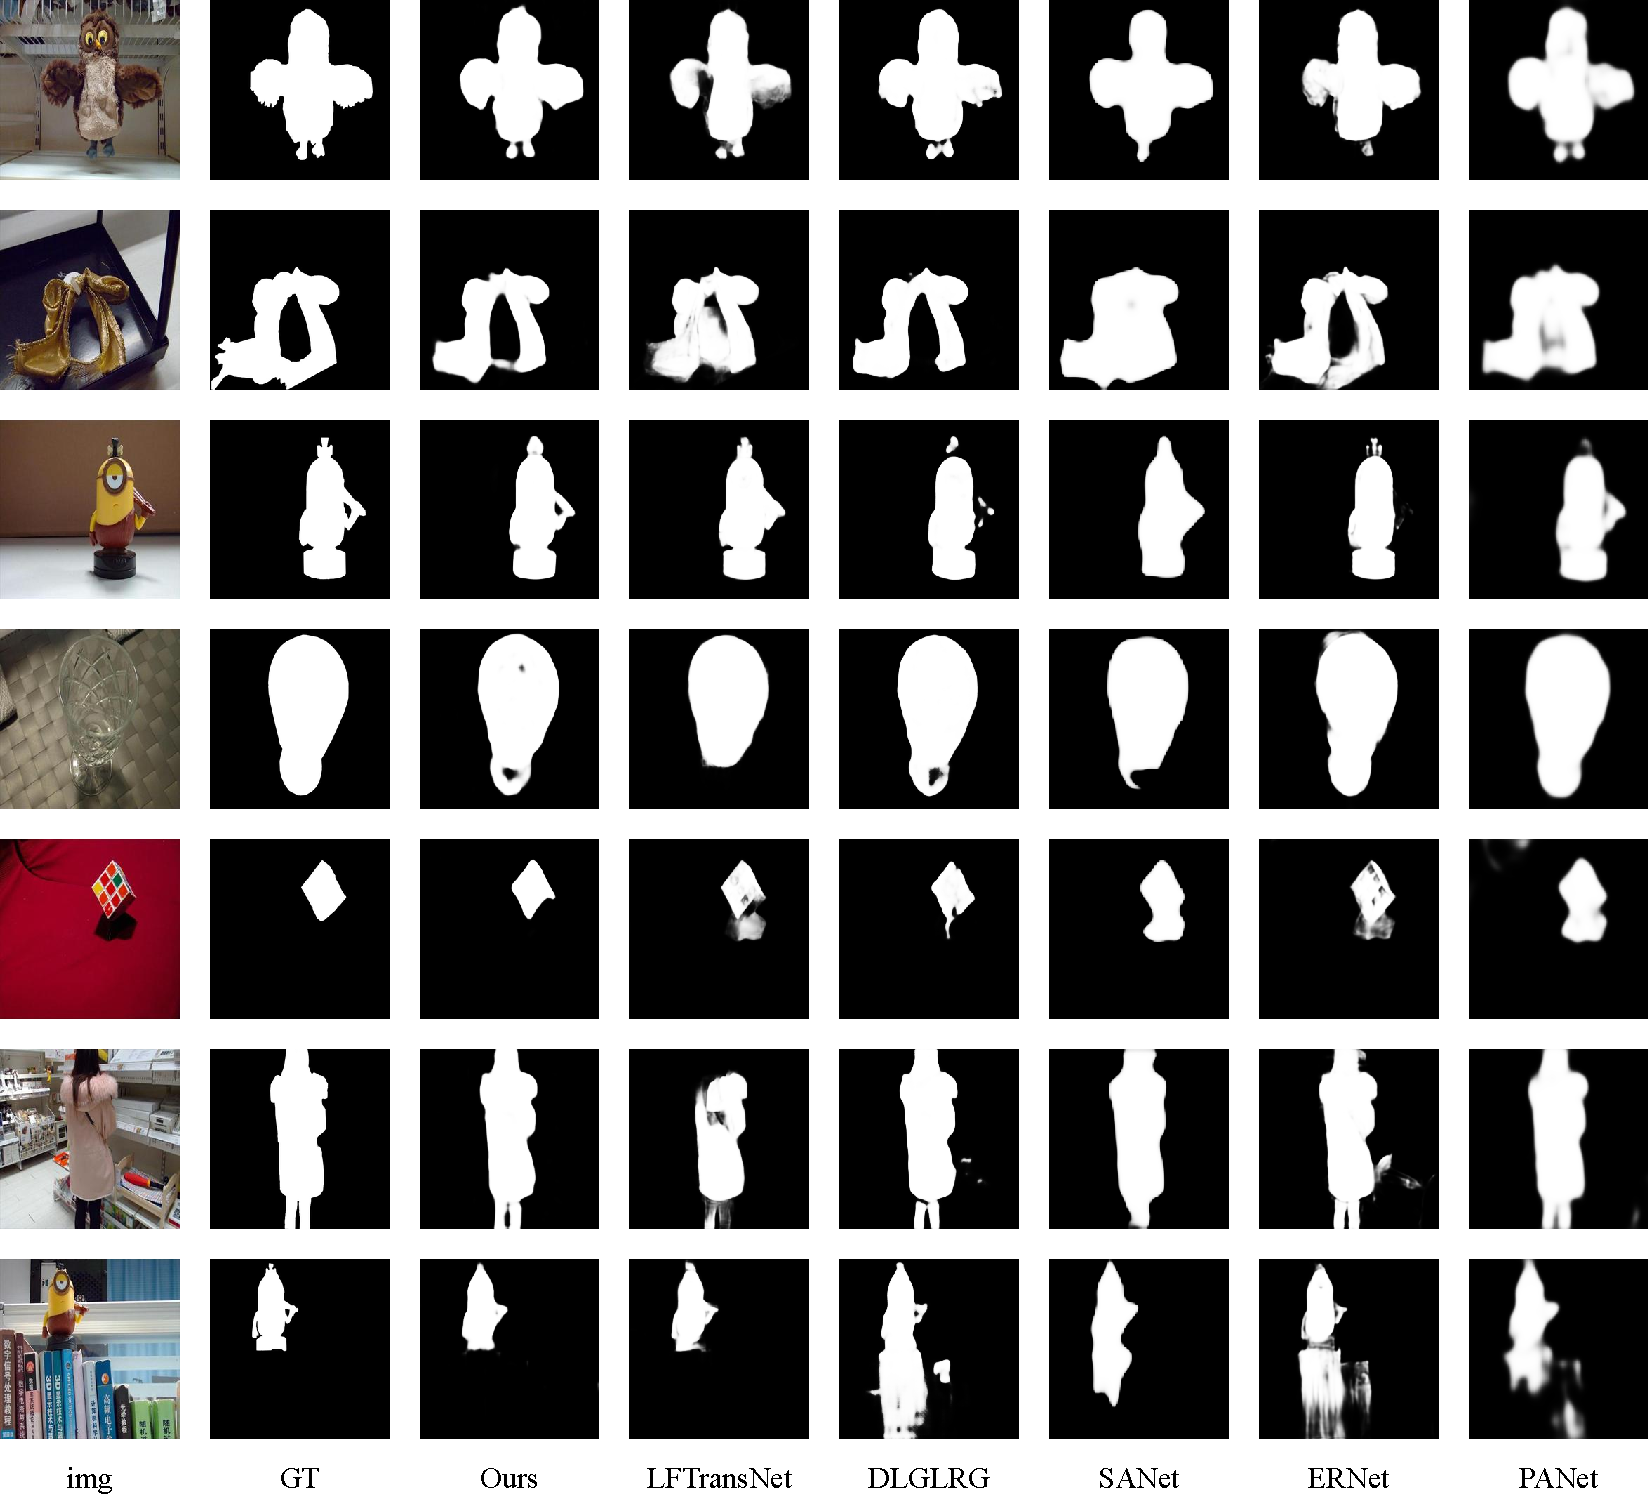
\includegraphics[width=\linewidth]{figures/chapter4/figures_comp}
	\bicaption{在不同场景下和现有方法的可视化定性比较}
	{Visual qualitative comparison with existing methods in various scenarios}
%	{与最先进方法的定性比较}
%	{Qualitative comparison with state-of-the-art methods}
%	{在一些具有挑战性的场景中与最先进的方法进行定性比较}
%	{Qualitative comparisons of state-of-the-art methods in some challenging scenes}
	\label{chpt4:fig:comparison_4}
\end{figure}



本节将本章方法与其他数据增强方法进行了比较。
为了进行全面比较,本节将本章方法与 27 个最先进的模型进行比较,
包括7个光场显著性分割方法:
LFTransNet \upcite{liu2023lftransnet},
DLGLRG \upcite{liu2021light}, RENet \upcite{piao2020exploit}, LFNet \upcite{zhang2020lfnet},
MAC \upcite{zhang2020light}, MoLF \upcite{zhang2019memory}, and DLSD \upcite{piao2019deep};
%
%
%
%
6个RGB-D显著性分割方法:
DCF \upcite{ji2021calibrated}, CIR-Net\upcite{cong2022cir}, VST-$rgbd$  \upcite{liu2021visual},
BBS-Net     \upcite{fan2020bbs}, SSF\upcite{zhang2020select} and S2MA    \upcite{liu2020learning};
%
%
%
%
%
和14个2D显著性检测方法:
VST-$rgb$ \upcite{liu2021visual},
PFSNet \upcite{ma2021pyramidal},
ITSD \upcite{zhou2020interactive},
LDF \upcite{wei2020label},
MINet \upcite{pang2020multi},
F$^{3}$Net  \upcite{wei2020f3net}, 
EGNet   \upcite{zhao2019egnet},
CPD  \upcite{wu2019cascaded},
PoolNet \upcite{liu2019simple},
PiCANet \upcite{liu2018picanet},
PAGRN \upcite{wang2018detect},
C2S   \upcite{li2018contour},
R3Net  \upcite{deng2018r3net}
和
Amulet \upcite{zhang2017amulet}。




为了保证公平比较,本章方法使用上述网络所公开提供的显着性预测图或预训练的权重来生成比较数据,
并利用\upcite{liu2021visual}中提供的相同评估代码。 
如表~\ref{chpt4:table:comp_with_sota_3_1}~所示,
很明显,所提出的方法在 DUTLF-FS 和 HFUT 数据集上实现了比当前最先进的方法更优越的性能。




%%%%%%%%%%%%%%%%%%%%%%%%%%%%%%%%%%%%%%%%%%%%%%%%%%%%%%%%%%%%%%%%%%%%%%%%%%%%%%%%%%%%%%%%%
(1)定性比较

图~\ref{chpt4:fig:comparison_4}~展示来本章方法与目前最先进的显著性目标检测方法在
不同场景的显著性预测的可视化效果。
在第1行中,本章方法能够更准确的预测出简单场景中显著性物体的边界。
举例来说,LFTransNet\upcite{liu2023lftransnet}和
\upcite{liu2021light}等光场显著性检测算法可以准确定位目标,
但是容易受到低对比度的背景噪声影响,从而无法得出完整的显著性预测。
图中第2行和第3行显示了网络能够在物体有轮廓的时候,
辨识出包含在显著性物体内部的非显著性区域,如领带的中间背景区域,
小黄人手臂和身体所围出的背景区域。
在一些困难场景下,比如透明物体(图中第4行),
本章方法能够辨识出与背景极为相似的显著性前景区域;
再如带有阴影区域的物体(图中第5行),本章所提的方法能够忽略物体影子的干扰,
做出正确的显著性检测。
图中第6行显示了在大物体场景下,本章所提方法能够注意到所有显著性的区域。
在有强干扰的场景下,如图中第7行,本章方法能够忽略同样清晰但是非显著书籍的干扰。
这些结果显示出本章所提出的基于视角增强模块的光场数据探索方法,能够更有效地利用多焦点数据,准确定位显著区域,
并在特征整合中突出显著区域、抑制非显著区域。


%
%
%在1-3行中,显著性目标在不同深度范围中表现突出;
%4-5行描述了多变的背景情况;
%6-7行展示了显著性目标与背景相近的挑战。本章方法可以准确且完整地预测这些复杂场景中的显著性目标。举例来说,EAR、LFNet和MOD等光场显著性检测算法可以准确定位目标,但无法完整预测;CPFP和PCA等RGB-D方法在有高质量深度图的场景中表现良好,但容易受到低质量深度图的干扰;CPD和PoolNet等RGB方法由于缺乏空间信息,在复杂场景中难以准确预测。
%这些结果显示出本章所提出的基于视角增强模块的光场数据探索方法,能够更有效地利用多焦点数据,准确定位显著区域,
%并在特征整合中突出显著区域、抑制非显著区域。
%
%




%%%%%%%%%%%%%%%%%%%%%%%%%%%%%%%%%%%%%%%%%%%%%%%%%%%%%%%%%%%%%%%%%%%%%%%%%%%%%%%%%%%%%%%%%%%%%%%%
(2)定量比较

表~\ref{chpt4:table:comp_with_sota_3_1}~展示了本章方法与现有方法在
DUTLF-FS、HFUT和LFSD三个数据集上的实验结果,
使用了E-measure、S-measure、F-measure和平均绝对误差四个评估指标来比较不同网络的性能。
表格以横线分割成了三部分,第一部分表示的是光场显著性检测网络的性能对比,
第二部分和第三部分分别是RGB-D显著性目标检测网络和RGB显著性目标检测网络在相应数据集上的泛化性能。
每一列性能的前三分别用加粗、红色以及蓝色字体表示。
本章方法在DUTLF-FS和HFUT两个数据集上的检测性能明显优于其他方法,并在DUTLF-FS上取得了与当前最有方法
LFTransNet\upcite{liu2023lftransnet}相媲美的性能,显著优于其他方法。
特别是在困难场景最多的的HFUT数据集上,
在E-measure指标上提升了3.8\%,
在平均绝对误差上降低了 16.1\%.
对E-measure指标的提升说明了,
与现有的光场显著性目标检测方法相比,本章可以生成与真值更加相似的预测图。







%%%%%%%%%%%%%%%%%%%%%%%%%%%%%%%%%%%%%%%%%%%%%%%%%%%%%%
\BiSection{本章总结}{The Chapter’s Conclusion}

本章提出了一种视角增强的光场显著性目标检测方法。
此方法主要包含一个视角增强模块和一个像素对比学习策略,
通过端到端的网络训练得到显著性预测图。
具体来说:
(1)
本章方法所提出的视角增强注意力模块,
能够充分提取隐含在全聚焦图和焦点堆栈
内部的场景显著信息,并促进两种不同光场场景表示的融合。
(2)
提出的像素对比监督,
能够考虑显著区域和非显著区域的内在联系,
使得网络对于显著区域有更为鲁棒的辨别能力。
广泛的实验结果表明,
本章方法相比现有的光场显著性分割方法,具有更优越的显著性分割性能。








